\FloatBarrier
\section{Query Modulated Sequential Benchmark \label{sec:additional-figures-query-mod-sequential}}

\begin{figure}[!htb]
% \vspace{-0.225in}
\centering
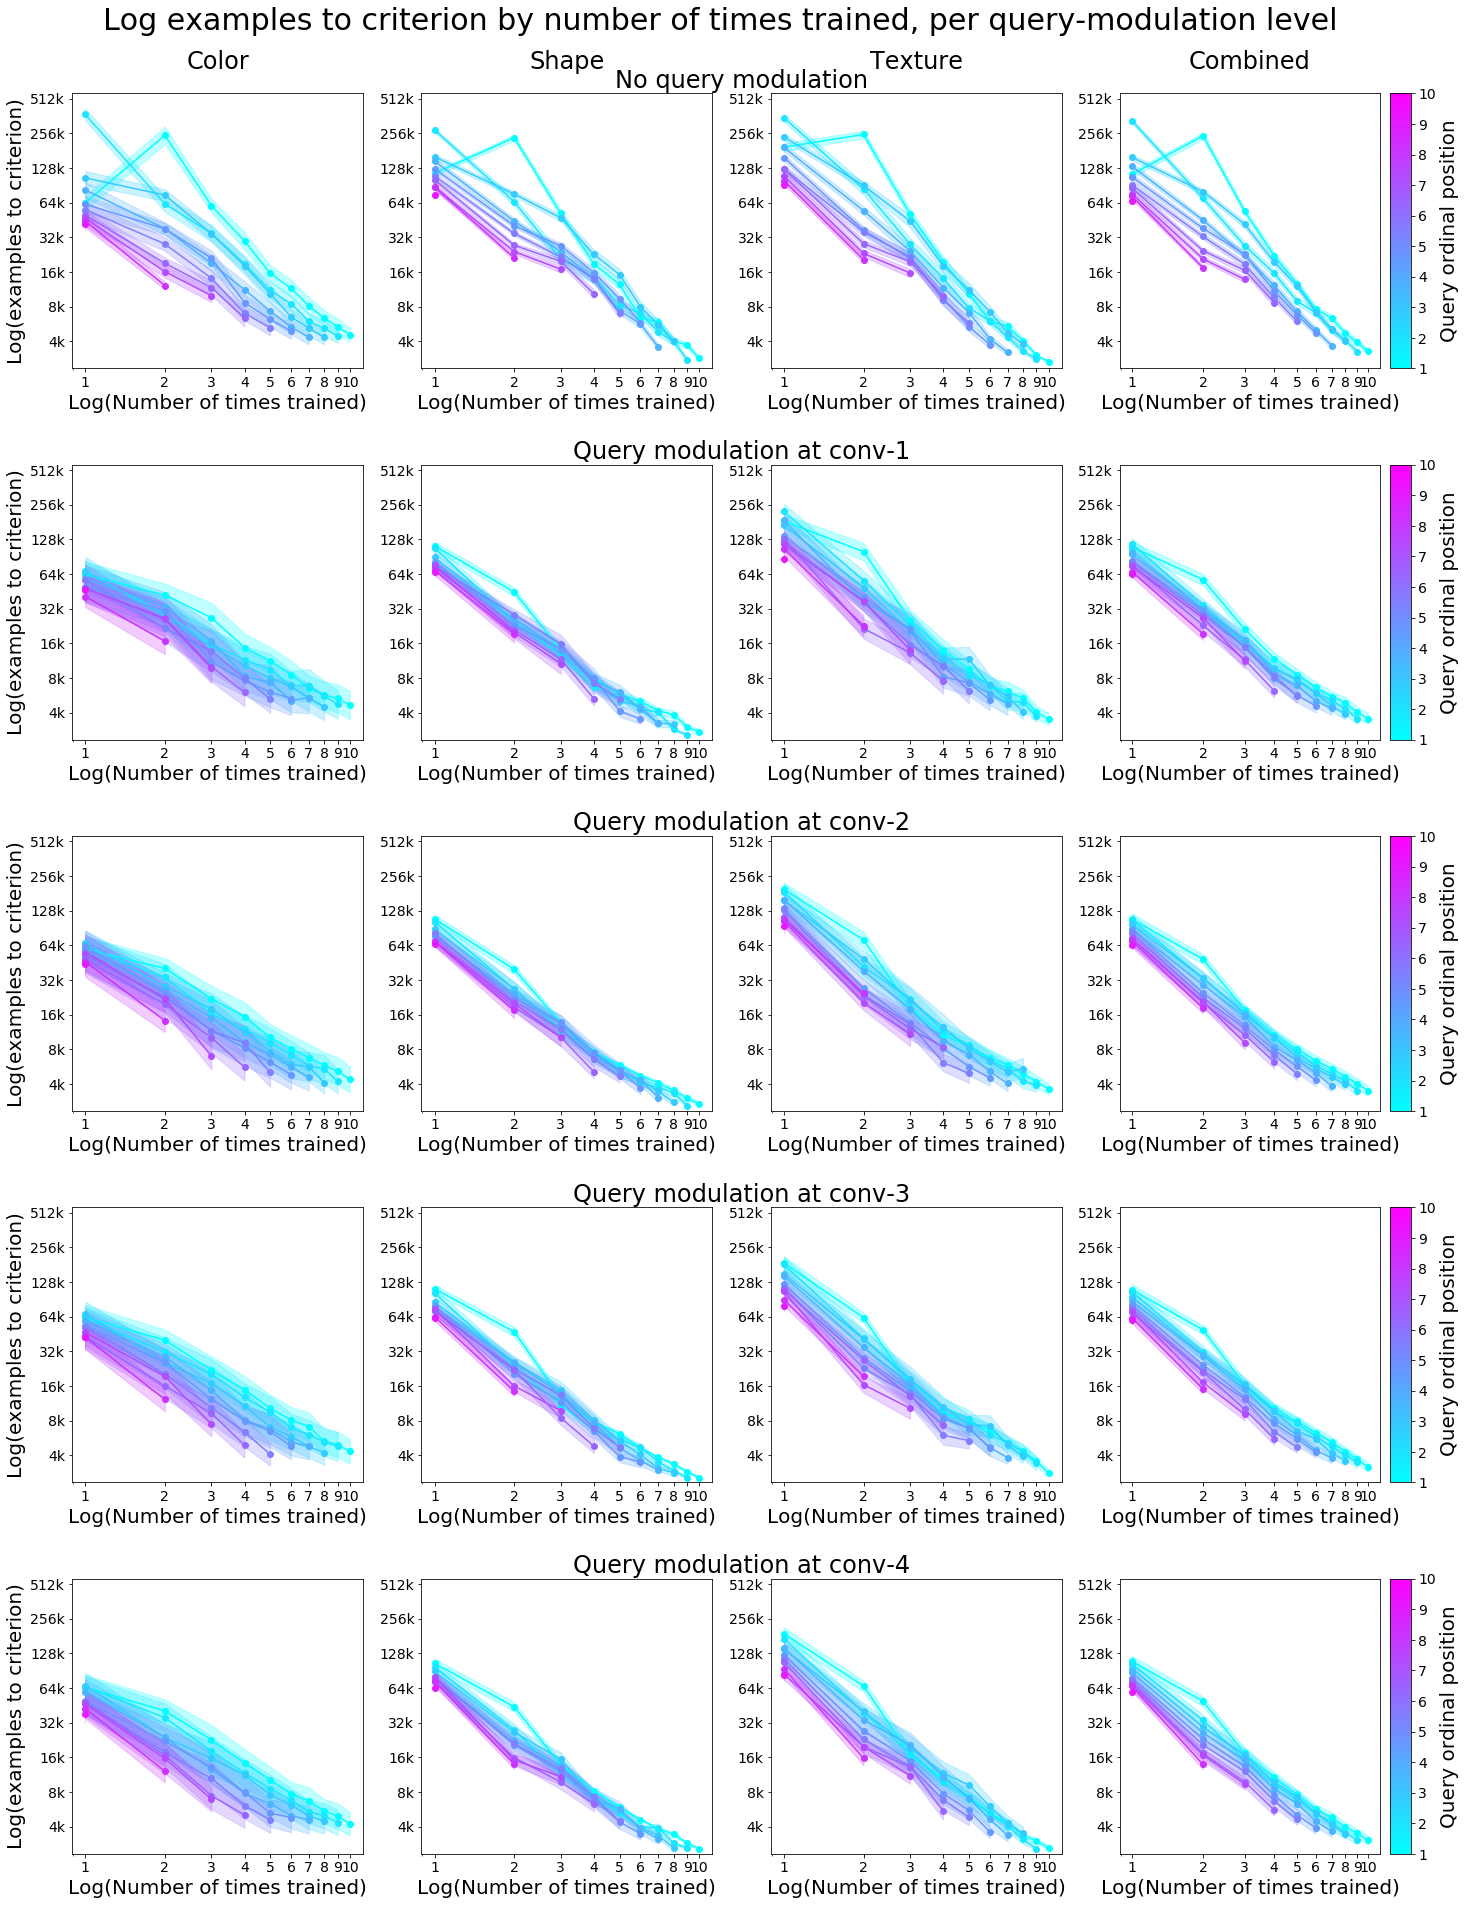
\includegraphics[width=\linewidth]{ch-results/figures/query_mod_benchmark/examples_to_criterion_per_modualtion_level_times_trained.png}
\caption[Log examples to criterion by number of times trained.]{ {\bf Log examples to criterion by number of times trained.} Split by each dimension and combined. All plots follow the same conventions as Figure \ref{fig:results-baseline-sequential-examples-to-criterion}: using a log-log scale to exhibit the power-law behavior, shading around the data reflects the standard errors of the mean (SEM), and the color scale reflects the order of query introduction, from the first query in the brightest cyan to the last query in the brightest pink.}
\label{fig:results-query-mod-benchmark-examples-to-criterion-per-modualtion-level-times-trained}
% \vspace{-0.2in}
\end{figure}

\begin{figure}[!htb]
% \vspace{-0.225in}
\centering
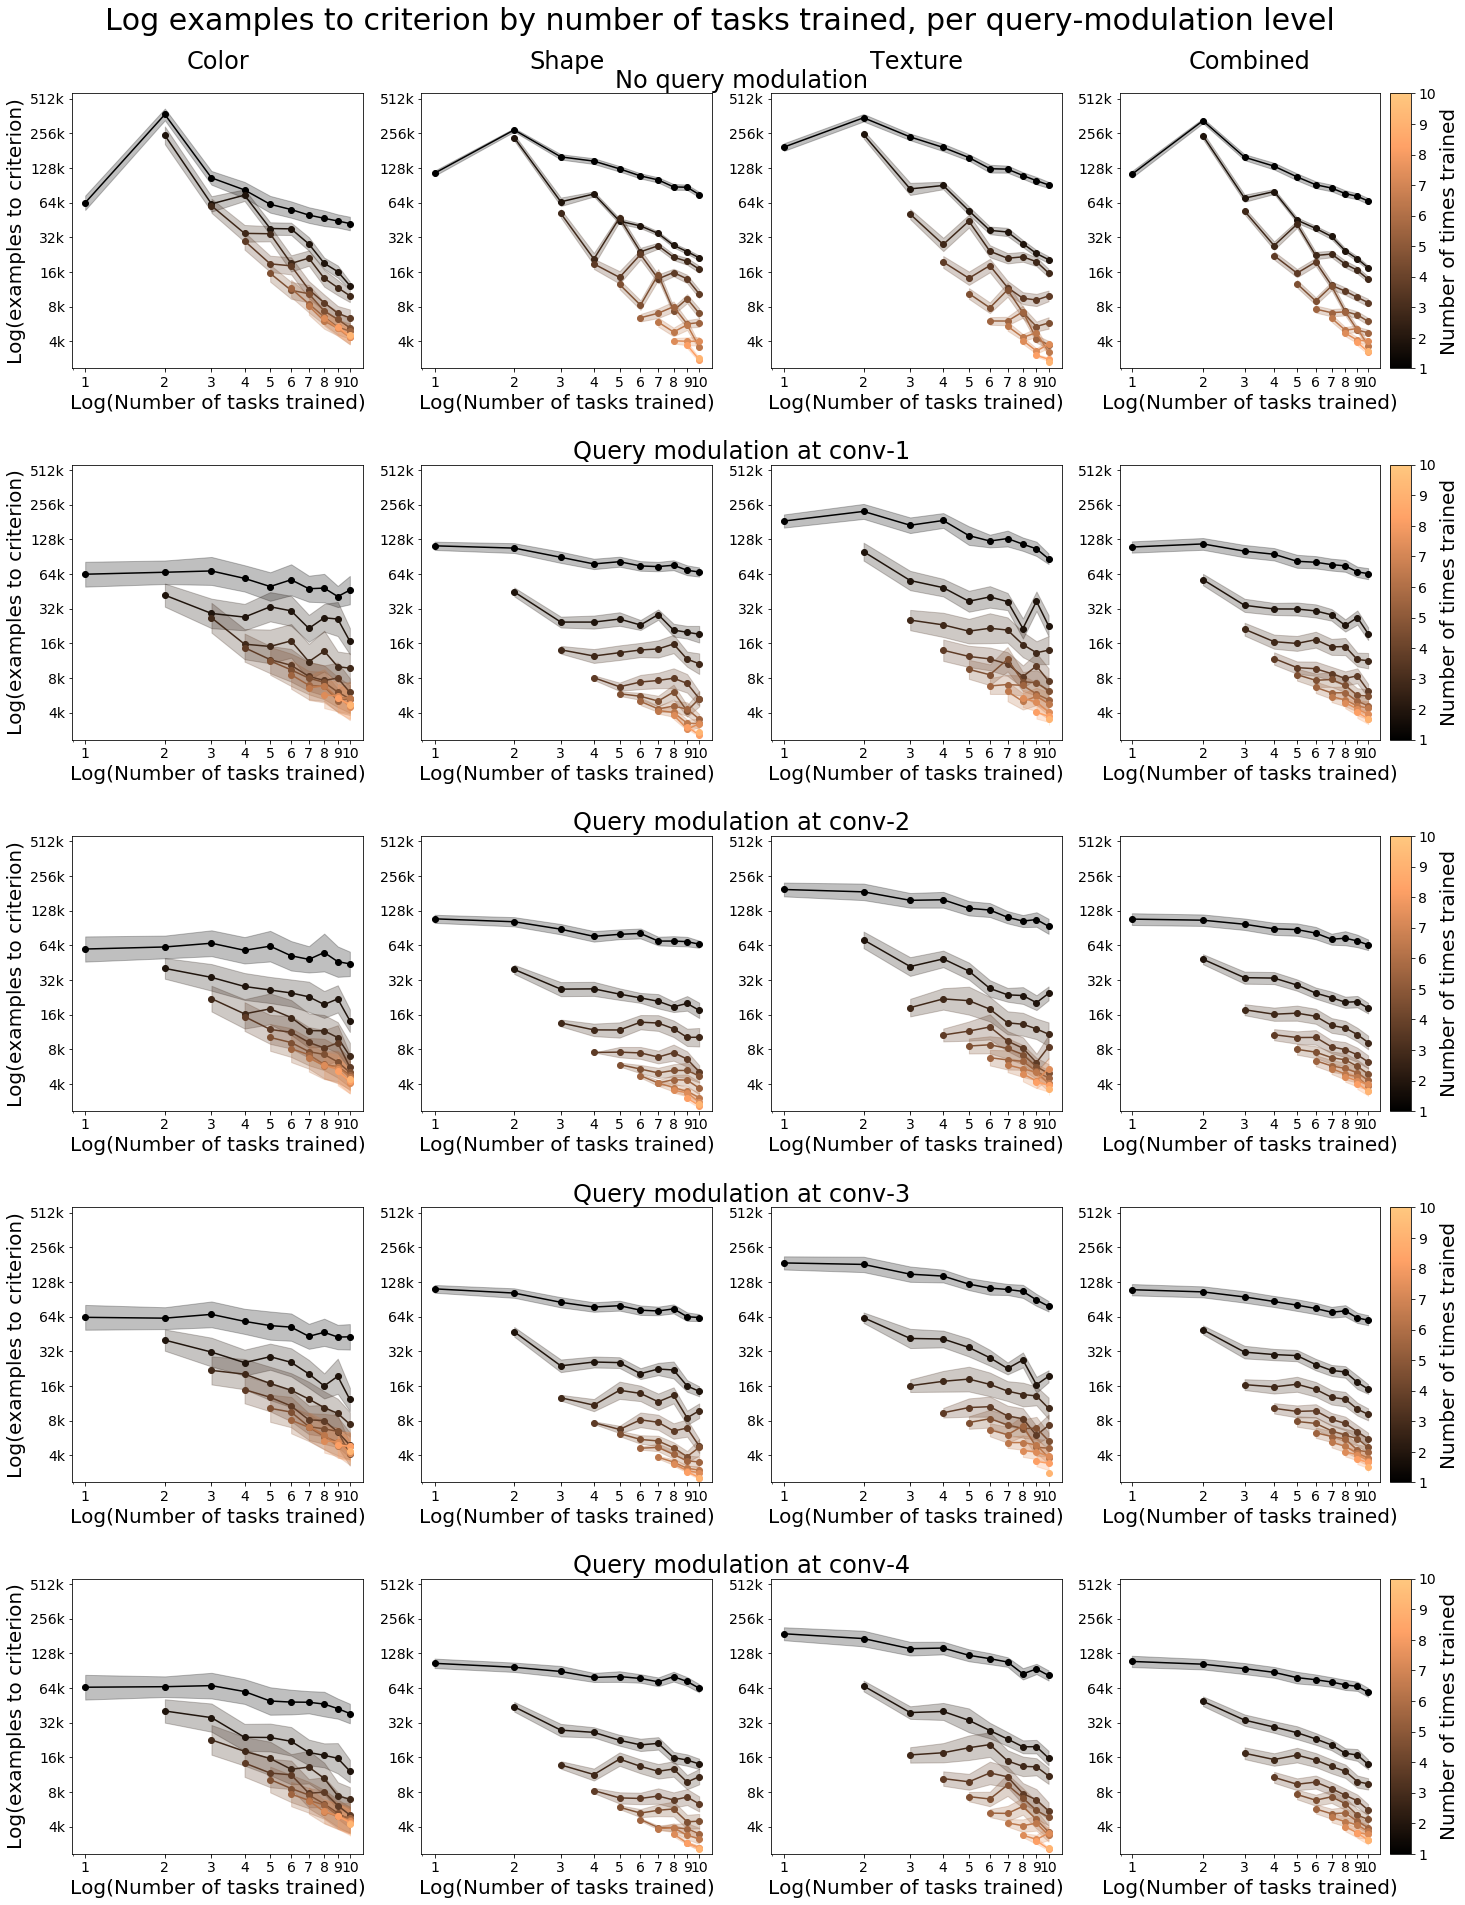
\includegraphics[width=\linewidth]{ch-results/figures/query_mod_benchmark/examples_to_criterion_per_modualtion_level_tasks_trained.png}
\caption[Log examples to criterion by number of tasks trained.]{ {\bf Log examples to criterion by number of tasks trained.} Split by each dimension and combined. All plots follow the same conventions as Figure \ref{fig:results-baseline-sequential-examples-to-criterion}: using a log-log scale to exhibit the power-law behavior, shading around the data reflects the standard errors of the mean (SEM), and the color scale reflects the order of query introduction, from queries trained on for the first time in black, to queries trained on for the tenth time in copper color.}
\label{fig:results-query-mod-benchmark-examples-to-criterion-per-modualtion-level-tasks-trained}
% \vspace{-0.2in}
\end{figure}

\begin{figure}[!htb]
% \vspace{-0.225in}
\centering
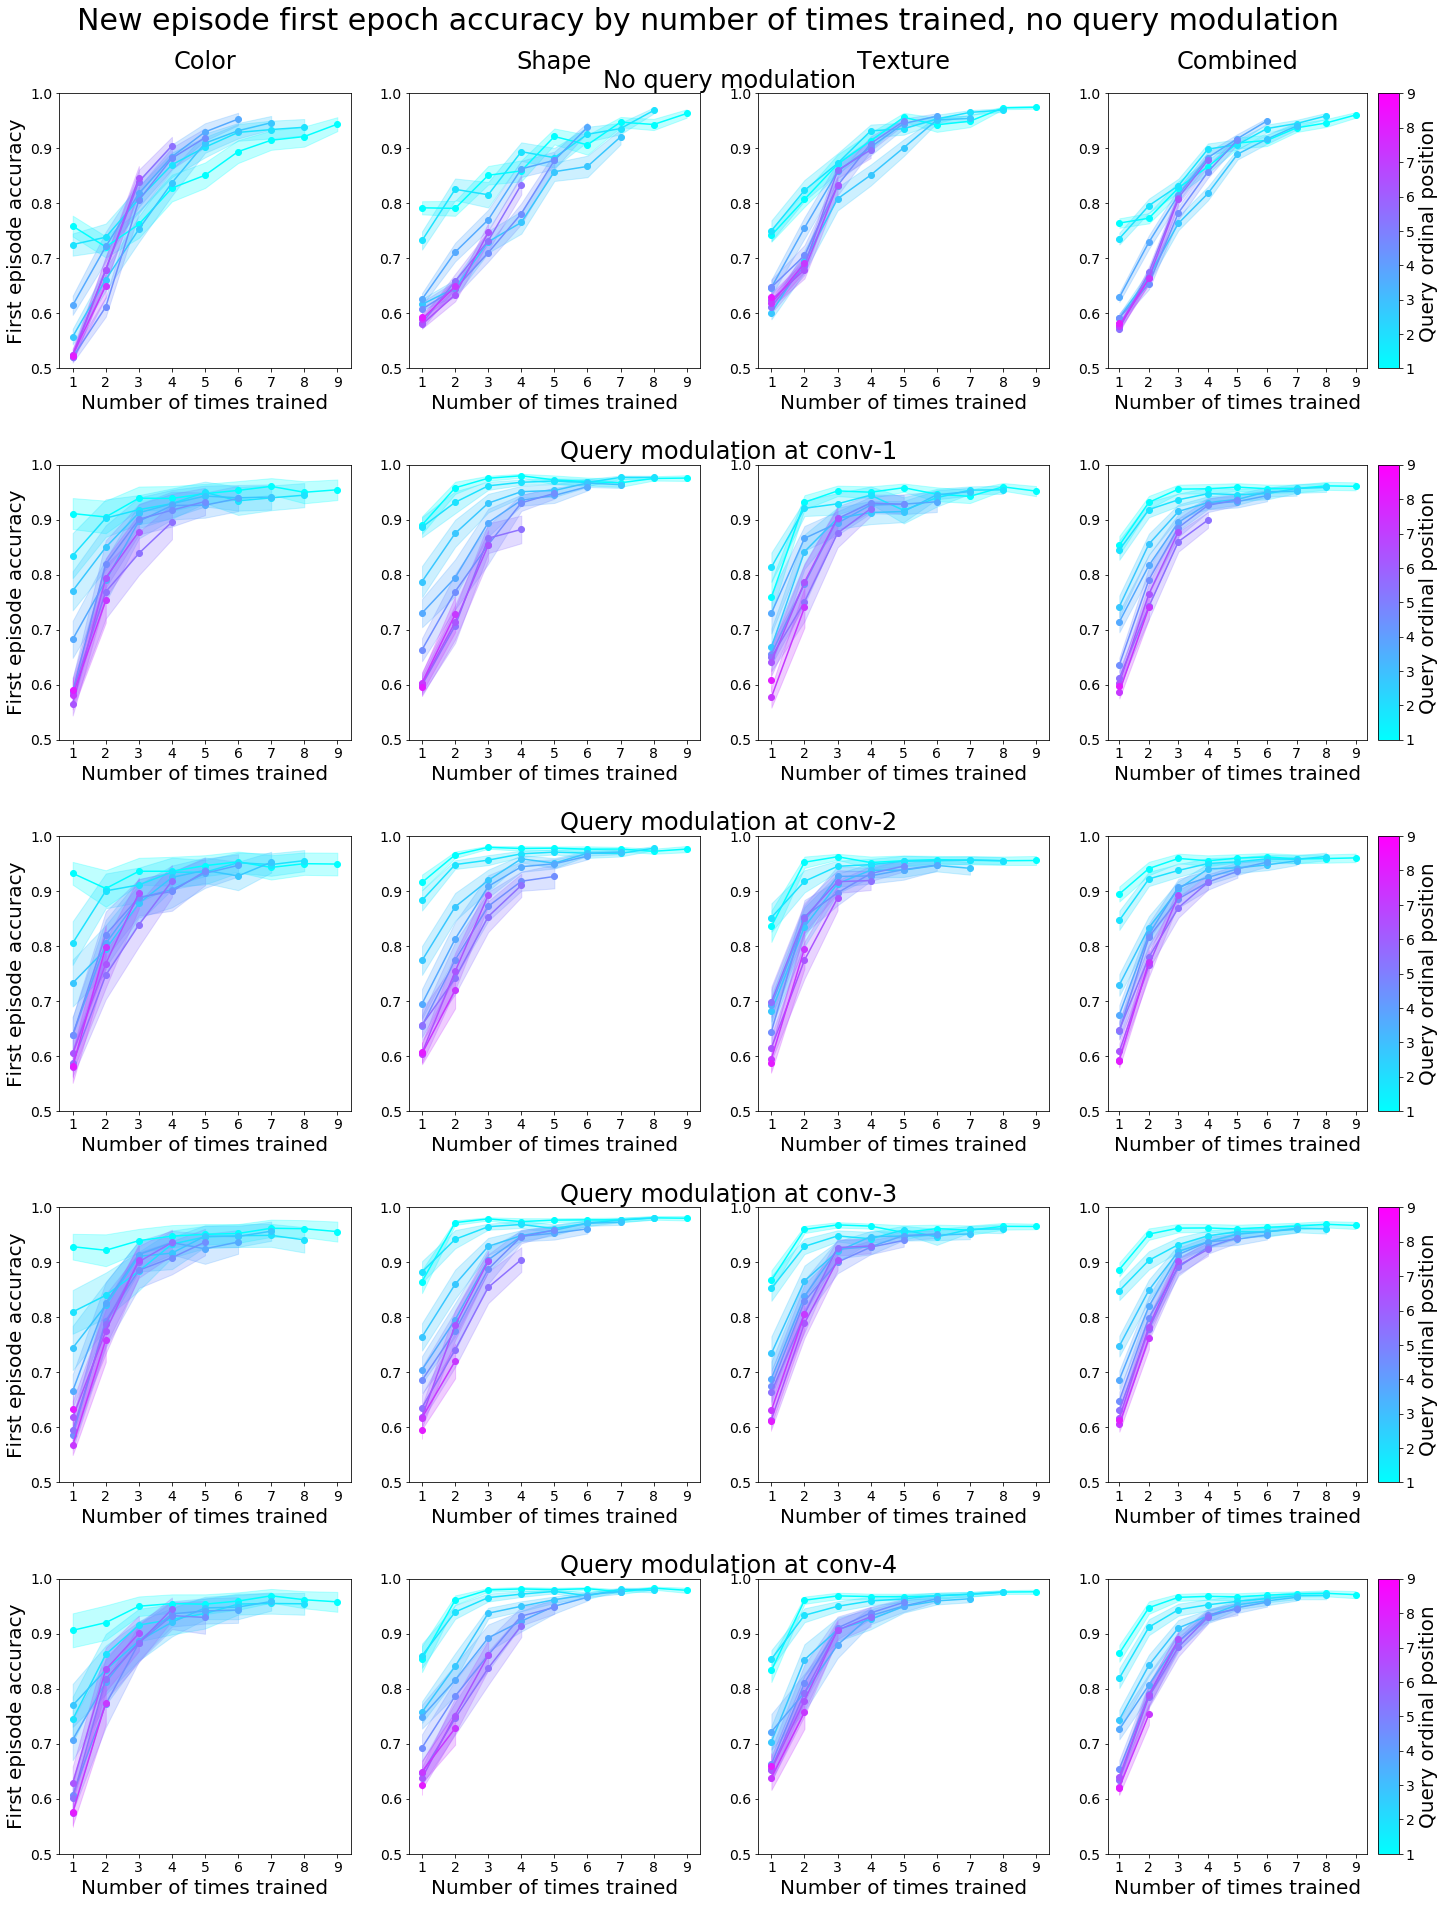
\includegraphics[width=\linewidth]{ch-results/figures/query_mod_benchmark/first_episode_accuracy_per_modualtion_level_times_trained.png}
\caption[New episode first epoch accuracy by number of times trained.]{ {\bf New episode first epoch accuracy by number of times trained.} Split by each dimension and combined. All plots follow the same conventions as Figure \ref{fig:results-baseline-sequential-examples-to-criterion}: using a log-log scale to exhibit the power-law behavior, shading around the data reflects the standard errors of the mean (SEM), and the color scale reflects the order of query introduction, from the first query in the brightest cyan to the last query in the brightest pink.}
\label{fig:results-query-mod-benchmark-first-episode-accuracy-per-modualtion-level-times-trained}
% \vspace{-0.2in}
\end{figure}

\begin{figure}[!htb]
% \vspace{-0.225in}
\centering
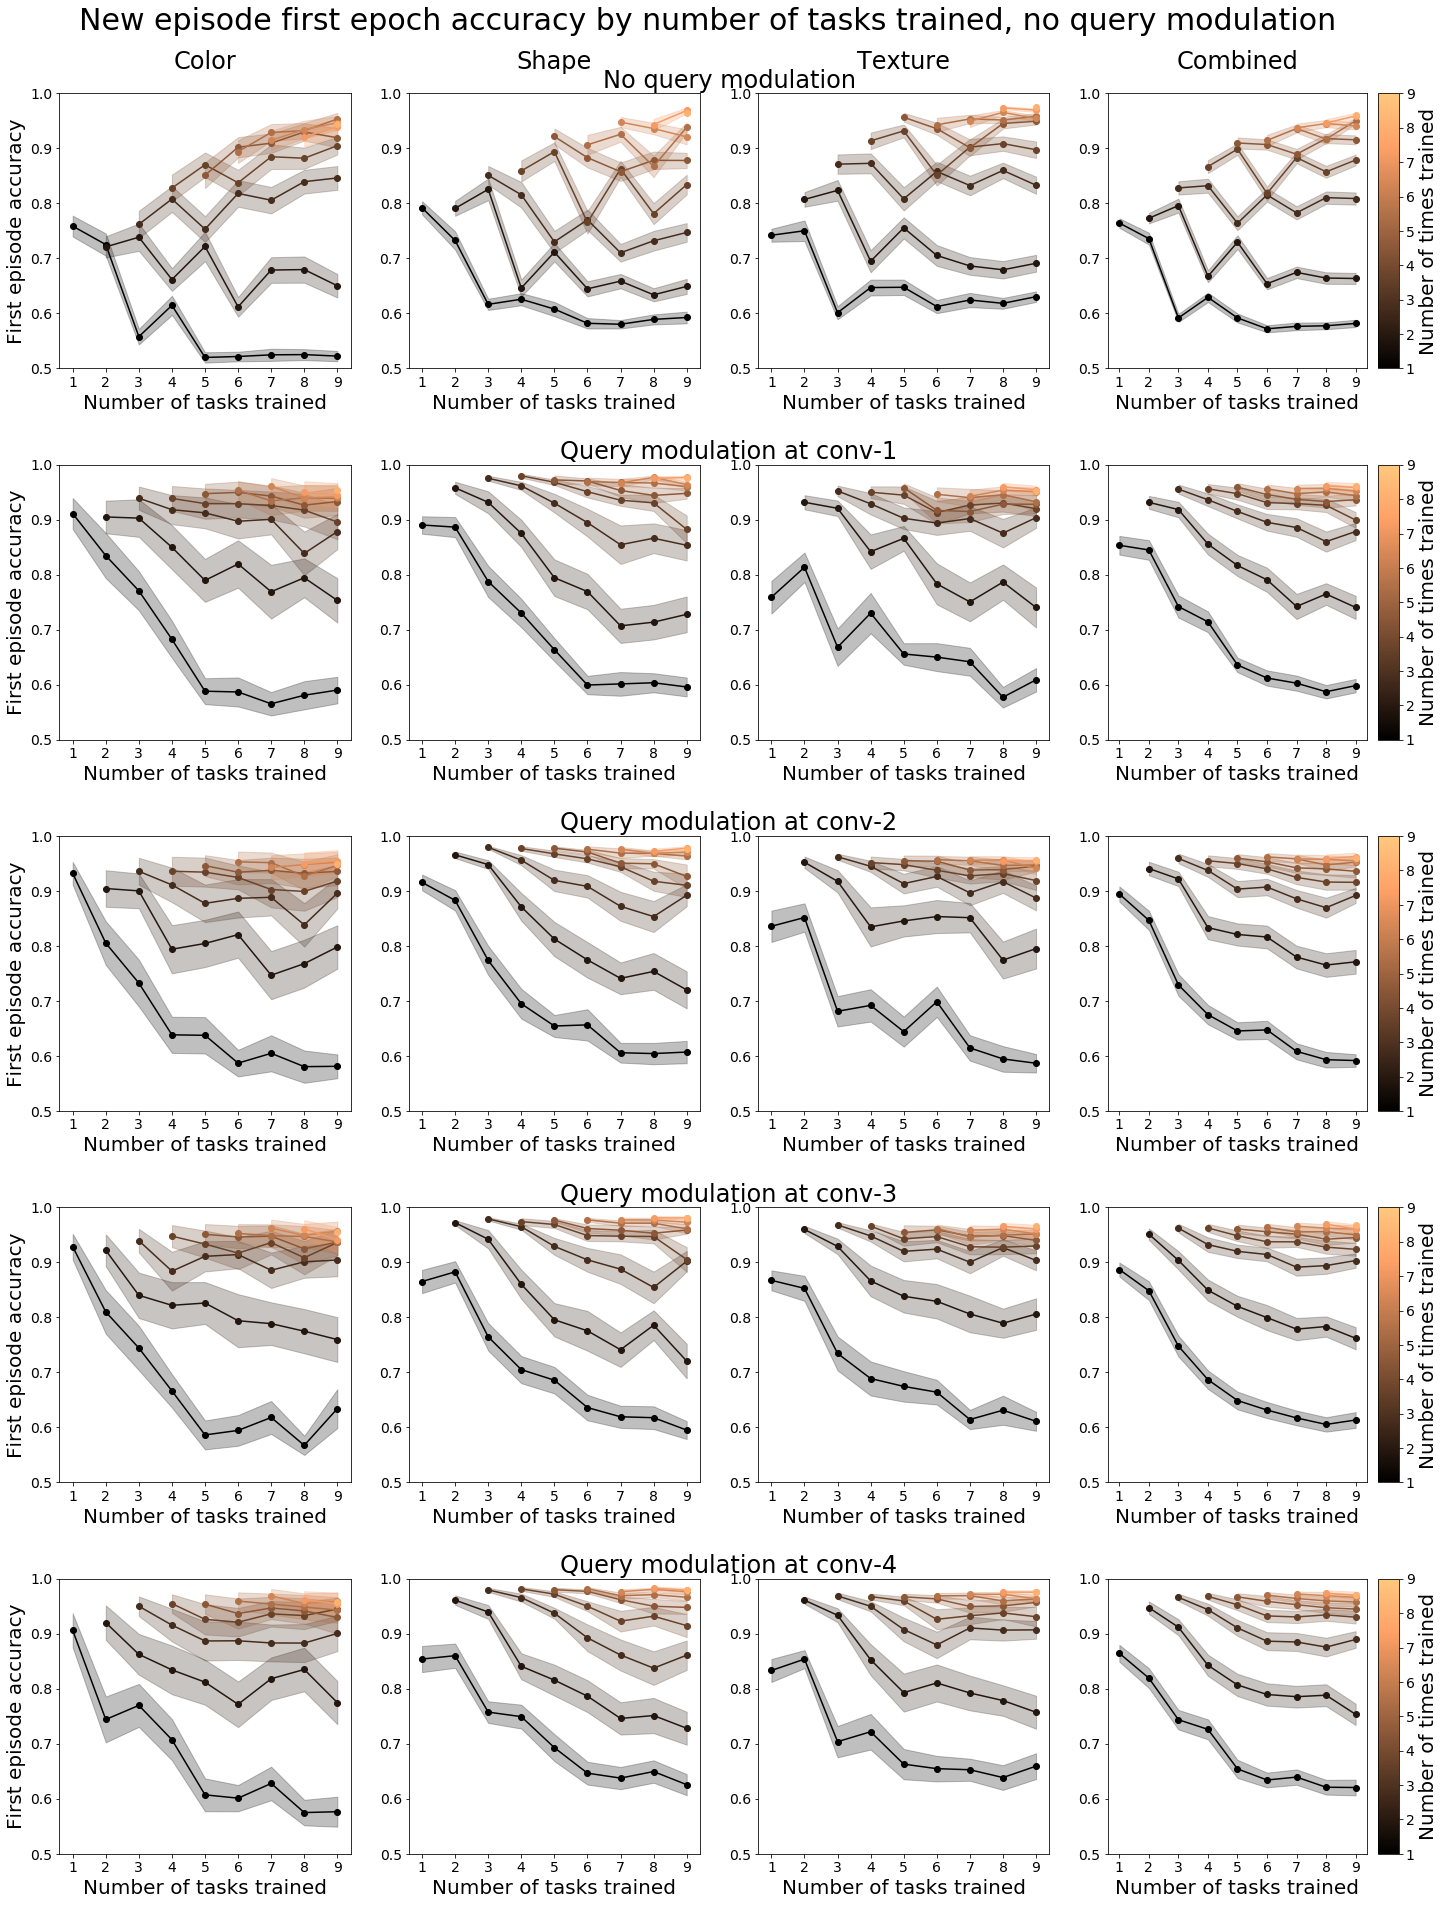
\includegraphics[width=\linewidth]{ch-results/figures/query_mod_benchmark/first_episode_accuracy_per_modualtion_level_tasks_trained.png}
\caption[New episode first epoch accuracy by number of tasks trained.]{ {\bf New episode first epoch accuracy by number of tasks trained.} Split by each dimension and combined. All plots follow the same conventions as Figure \ref{fig:results-baseline-sequential-examples-to-criterion}: using a log-log scale to exhibit the power-law behavior, shading around the data reflects the standard errors of the mean (SEM), and the color scale reflects the order of query introduction, from queries trained on for the first time in black, to queries trained on for the tenth time in copper color. }
\label{fig:results-query-mod-benchmark-first-episode-accuracy-per-modualtion-level-tasks-trained}
% \vspace{-0.2in}
\end{figure}
